\documentclass{article}
\usepackage[
  margin = 1in,
]{geometry}
\usepackage{amsmath, amssymb}
\usepackage{enumitem}
\usepackage{bm}
\usepackage{tikz}

\begin{document}

\section*{Problem}
\begin{enumerate}[label=\fbox{\arabic*}]
  \item Let $K$ be the minimal splitting field of the polynomial $f(X) = X^4 - 2X^2 - 2$ over $\mathbb{Q}$. Answer the following questions.
        \begin{enumerate}[label=(\arabic*)]
          \item Determine the Galois group $\operatorname{Gal}(K/\mathbb{Q})$.
          \item Determine all intermediate fields $F$ of $K/\mathbb{Q}$ such that $f(X)$ is irreducible as a polynomial over $F$.
        \end{enumerate}

  \item Let $\mathbb{C}[X, Y, Z]$ be the polynomial ring in three variables over $\mathbb{C}$. We define the ideal $I$ of $\mathbb{C}[X, Y, Z]$ by
        \[
          I = (X^2Y + Z^2, X^4 - Y^3 + 2XYZ).
        \]
        Answer the following questions.
        \begin{enumerate}[label=(\arabic*)]
          \item We define the subsets $V, W$ of $\mathbb{C}^3$ by
                \begin{align*}
                  V & = \{ (a, b, c) \in \mathbb{C}^3 \mid f(a, b, c) = 0 \text{ for every } f \in I \}, \\
                  W & = \{ (t^3, -t^4, t^5) \in \mathbb{C}^3 \mid t \in \mathbb{C} \}.
                \end{align*}
                Determine whether or not $V$ is equal to $W$.
          \item Let $J$ be the radical of $I$. Determine whether or not $\mathbb{C}[X, Y, Z]/J$ is a unique factorization domain (UFD).
        \end{enumerate}

  \item Let $S^3 = \{ (x, y, z, w) \in \mathbb{R}^4 \mid x^2 + y^2 + z^2 + w^2 = 1 \}$. We define an open set $U$ of $S^3$ and submanifolds $L, M$ of $S^3$ by
        \begin{align*}
          U & = \left\{ (x, y, z, w) \in S^3 \;\middle|\; x^2 + y^2 > \frac{1}{2} \right\}, \\
          L & = \{ (x, y, z, w) \in S^3 \mid z = w = 0 \},                                  \\
          M & = \{ (x, y, z, w) \in S^3 \mid x = y = 0 \}.
        \end{align*}
        We assume that $L$ is oriented.
        \begin{enumerate}[label=(\arabic*)]
          \item Prove that there exists a $C^\infty$ 1-form $\eta$ on $S^3$ satisfying
                \[
                  d\eta|_U = 0, \quad \int_L \eta = 1. \qquad (*)
                \]
                Here $d\eta|_U$ is the restriction of $d\eta$ to $U$.
          \item Let $\eta$ be a $C^\infty$ 1-form on $S^3$ that satisfies the condition $(*)$. Prove that the following statement holds for suitable choices of the orientations of $S^3$ and $M$.
                If a $C^\infty$ 1-form $\xi$ on $S^3$ satisfies $\operatorname{supp}(d\xi) \subset U$, then we have
                \[
                  \int_{S^3} d\eta \wedge \xi = \int_M \xi.
                \]
                Here $\operatorname{supp}(d\xi)$ is the closure of $\{ p \in S^3 \mid (d\xi)_p \neq 0 \}$.
        \end{enumerate}

  \item We set $S = \{ \boldsymbol{x} \in \mathbb{R}^3 \mid \|\boldsymbol{x}\| = 1 \}$, where $\|\boldsymbol{x}\|$ is the standard norm of $\boldsymbol{x}$ in $\mathbb{R}^3$. We define a subspace $E$ of $S \times S$ by
        \[
          E = \{ (\boldsymbol{x}, \boldsymbol{y}) \in S \times S \subset \mathbb{R}^3 \times \mathbb{R}^3 \mid \boldsymbol{x} \cdot \boldsymbol{y} = 0 \},
        \]
        where $\boldsymbol{x} \cdot \boldsymbol{y}$ is the standard inner product of $\boldsymbol{x}$ and $\boldsymbol{y}$ in $\mathbb{R}^3$.
        \begin{enumerate}[label=(\arabic*)]
          \item Compute the homology groups of $E$ with integer coefficients.
          \item We define a map $\pi: E \to S$ by $\pi(\boldsymbol{x}, \boldsymbol{y}) = \boldsymbol{x}$. We define a subspace $F$ of $E \times E$ by
                \[
                  F = \{ (e_1, e_2) \in E \times E \mid \pi(e_1) = \pi(e_2) \}.
                \]
                Compute the homology groups of $F$ with integer coefficients.
        \end{enumerate}

  \item Let $(X, \mathcal{M}, \mu)$ be a measure space, and set
        \[
          \|h\|_r = \left( \int_X |h|^r d\mu \right)^{1/r}
        \]
        for each $\mathcal{M}$-measurable function $h: X \to \mathbb{C}$ and $r \in (1, \infty)$. Let $p \in (1, \infty)$, set $q = \frac{p}{p-1}$, and suppose that a sequence $\{f_n\}_{n=1}^\infty$ of $\mathcal{M}$-measurable functions $f_n: X \to \mathbb{C}$ and an $\mathcal{M}$-measurable function $f: X \to \mathbb{C}$ satisfy the following conditions (A), (B) and (C):
        \begin{enumerate}[label=({\Alph*})]
          \item $\lim_{n\to\infty} f_n(x) = f(x)$ for $\mu$-a.e. $x \in X$.
          \item $\|f_n\|_p < \infty$ for any positive integer $n$.
          \item For any $\mathcal{M}$-measurable function $g: X \to \mathbb{C}$ satisfying $\|g\|_q < \infty$, it holds that
                \[
                  \lim_{n\to\infty} \int_X f_n g \, d\mu = 0.
                \]
        \end{enumerate}
        Answer the following questions.
        \begin{enumerate}[label=(\arabic*)]
          \item Show that $\|f\|_p \le \sup_{n \ge 1} \|f_n\|_p < \infty$.
          \item Let $E \in \mathcal{M}$ satisfy $\mu(E) < \infty$. Show that
                \[
                  \lim_{n\to\infty} \int_E f_n \, d\mu = \int_E f \, d\mu.
                \]
          \item Show that $f(x) = 0$ for $\mu$-a.e. $x \in X$.
        \end{enumerate}

  \item Let $X$ be an infinite-dimensional real Banach space, and let $\mathbb{K}$ be the real vector space of compact linear operators from $X$ to $X$. For each bounded linear operator $T$ from $X$ to $X$, let $\|T\|$ denote the operator norm of $T$.
        \begin{enumerate}[label=(\arabic*)]
          \item Let $T_n \in \mathbb{K}$ for each positive integer $n$, let $T$ be a bounded linear operator from $X$ to $X$, and suppose that $\lim_{n\to\infty} \|T_n - T\| = 0$. Show that $T \in \mathbb{K}$.
          \item Let $L$ and $R$ be linear maps from $\mathbb{K}$ to $\mathbb{K}$. Suppose that
                \[
                  S L(T) = R(S) T
                \]
                for all $S, T \in \mathbb{K}$. Show that $L$ is a bounded linear operator from the normed space $(\mathbb{K}, \|\cdot\|)$ to itself.
        \end{enumerate}

  \item Define sets $X$ and $Y$ as follows:
        \begin{align*}
          X & = \left\{ f \;\middle|\; \begin{array}{l} f: [0, \infty) \times [0, \pi] \to \mathbb{R} \text{ is continuous, } \\ f \text{ is } C^2 \text{ for } (t, x) \in (0, \infty) \times (0, \pi), \text{ and} \\ \frac{\partial f}{\partial t}, \frac{\partial f}{\partial x} \text{ and } \frac{\partial^2 f}{\partial x^2} \text{ are extended to} \\ \text{real valued continuous functions on } [0, \infty) \times [0, \pi] \end{array} \right\}, \\
          Y & = \left\{ g \;\middle|\; \begin{array}{l} g: [0, \pi] \to \mathbb{R} \text{ is continuous, } g \text{ is } C^3 \text{ on } (0, \pi), \\ g', g'' \text{ and } g''' \text{ are extended to} \\ \text{real valued continuous functions on } [0, \pi] \end{array} \right\}.
        \end{align*}
        Answer the following questions.
        \begin{enumerate}[label=(\arabic*)]
          \item Let $u_0 \in Y$ satisfy $u_0'(0) = u_0'(\pi) = 0$. Show that there exists a unique element $u$ of $X$ satisfying the following:
                \[
                  \begin{cases} \frac{\partial u}{\partial t}(t, x) = \frac{\partial^2 u}{\partial x^2}(t, x) + u(t, x), & t > 0, \; 0 < x < \pi, \\ \frac{\partial u}{\partial x}(t, 0) = \frac{\partial u}{\partial x}(t, \pi) = 0, & t \ge 0, \\ u(0, x) = u_0(x), & 0 \le x \le \pi. \end{cases} \qquad \text{(A)}
                \]
          \item Let $\alpha \in (0, \infty)$ and $w_0 \in Y$ satisfy $w_0'(0) = \alpha$, $w_0'(\pi) = -\alpha$, and the following:
                \[
                  \int_0^\pi w_0(y) \, dy = 2\alpha, \quad \int_0^\pi w_0(y) \cos y \, dy = 0. \qquad \text{(B)}
                \]
                Furthermore, let $w \in X$ satisfy the following:
                \[
                  \begin{cases} \frac{\partial w}{\partial t}(t, x) = \frac{\partial^2 w}{\partial x^2}(t, x) + w(t, x), & t > 0, \; 0 < x < \pi, \\ \frac{\partial w}{\partial x}(t, 0) = \alpha, \quad \frac{\partial w}{\partial x}(t, \pi) = -\alpha, & t \ge 0, \\ w(0, x) = w_0(x), & 0 \le x \le \pi. \end{cases} \qquad \text{(C)}
                \]
                Show that there exist a constant $C \in (0, \infty)$ and $\phi \in Y$ such that
                \[
                  |w(t, x) - \phi(x)| \le C e^{-3t}
                \]
                for any $(t, x) \in [0, \infty) \times [0, \pi]$.
        \end{enumerate}

  \item Let $a \in \mathbb{R}$. Consider the following differential equations for real-valued functions $x(t), y(t), z(t)$ with respect to time $t \in \mathbb{R}$,
        \[
          (*) \begin{cases} \frac{dx}{dt} = ax + y + yz, \\ \frac{dy}{dt} = x + ay + zx, \\ \frac{dz}{dt} = az - 2xy. \end{cases}
        \]
        Answer the following questions.
        \begin{enumerate}[label=(\arabic*)]
          \item Let $V: \mathbb{R}^3 \to \mathbb{R}$ be a function, given by
                \[
                  V(x, y, z) = \frac{1}{2}(x^2 + y^2 + z^2).
                \]
                Show that there exists a constant $C$ such that for any $t \in \mathbb{R}$, the inequality
                \[
                  \frac{d}{dt}V(x(t), y(t), z(t)) \le CV(x(t), y(t), z(t))
                \]
                holds.
          \item Show that for any initial values and any $a \in \mathbb{R}$, the solutions of the differential equations $(*)$ do not blow up at a finite time.
          \item Find the condition on $a$ such that the origin $(x, y, z) = (0, 0, 0)$ is linearly stable.
          \item When the origin $(x, y, z) = (0, 0, 0)$ is linearly stable, show that all solutions of the differential equations $(*)$ converge to the origin as $t \to \infty$.
        \end{enumerate}

  \item Let us consider sedimentation of small particles. These particles are sufficiently heavier than the surrounding fluid. The forces of gravity and resistance are balanced for each particle. The interactions between particles are ignored.
        \begin{enumerate}[label=(\arabic*)]
          \item Take the $x$ axis to denote the vertical upward direction and assume that gravity operates in the negative $x$ direction. Let us denote the particle mass by $m$, the upward velocity by $u$, the resistance by $-\gamma u$ and the gravity by $-mg(x)$, where $m$ and $\gamma$ are positive constants. Write an equation determining the motion of each particle.
        \end{enumerate}
        Suppose that $g(x) = g_0 x$, where $g_0$ is a positive constant.
        \begin{enumerate}[label=(\arabic*), resume]
          \item Find the position of the particle $x(t)$, and its velocity $u(t)$, using the constant, $\alpha = m g_0 / \gamma$. Here, $t$ is time, and the position at $t = 0$ is defined as $x(0) = \xi > 0$.
          \item Suppose that the particle's number density, $\rho(x, t)$, obeys the following equation:
                \[
                  \frac{\partial \rho}{\partial t} + \frac{\partial}{\partial x}(\rho u) = 0.
                \]
                Here, $u$ denotes the velocity obtained in (2). Furthermore, we assume $\rho(0, t) = \rho(\infty, t) = 0$ by supposing that the particles concentrate around a certain height. Then, show the relation
                \[
                  \frac{d}{dt} \int_0^\infty \rho(x, t) \, dx = 0.
                \]
          \item When the initial distribution is given as $\rho(x, 0) = f(x)$, obtain the distribution at time $t$, $\rho(x, t)$, by performing the coordinate transformation from $(x, t)$ to $(\xi, \tau)$, where $x = \xi e^{-\alpha \tau}$ and $t = \tau$.
          \item Assuming that the initial distribution $f(x)$ is shown as in the figure below, explain how the $x$-profile of the number density $\rho$ evolves over time by drawing a graph.
                \begin{center}
                  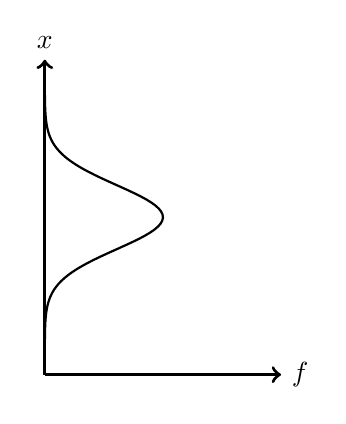
\begin{tikzpicture}[scale=1]
                    \draw[->, very thick] (0, 0) -- (3, 0) node[right] {$f$};
                    \draw[->, very thick] (0, 0) -- (0, 4) node[above] {$x$};
                    \draw[thick, domain=0:3.8, samples=100] plot ({1.5*exp(-3*(\x-2)^2)}, \x);
                  \end{tikzpicture}
                \end{center}
        \end{enumerate}

  \item \begin{enumerate}[label=(\arabic*)]
          \item We write $\mathbb{N}$ for the set of nonnegative integers. Let $(A, <_A)$ be a well-ordered set. Define $M(A)$ to be the set of functions $t: A \to \mathbb{N}$ such that $t(a) = 0$ for all but finitely many $a \in A$. Define a binary relation $<_{M(A)}$ on $M(A)$ by
                \[
                  t <_{M(A)} u \iff \begin{array}{l} \text{there exists some } a \in A \text{ such that } t(a) < u(a) \\ \text{and } t(a') = u(a') \text{ for every } a' >_A a. \end{array}
                \]
                Prove that $(M(A), <_{M(A)})$ is a well-ordered set.
          \item Consider the following operations on a list $\ell = [m_1, m_2, \dots, m_k]$ of nonnegative integers and a nonnegative integer $n$:
                \begin{align*}
                  \mathbf{len}(\ell)     & = k,                         \\
                  \mathbf{cons}(n, \ell) & = [n, m_1, m_2, \dots, m_k], \\
                  \mathbf{hd}(\ell)      & = m_1,                       \\
                  \mathbf{tl}(\ell)      & = [m_2, \dots, m_k],
                \end{align*}
                where $\mathbf{hd}(\ell)$ and $\mathbf{tl}(\ell)$ are undefined when $\ell$ is the empty list. Prove that the following program halts for any list $\ell$ of nonnegative integers.
                \begin{center}
                  \begin{minipage}{0.7\textwidth}
                    \begin{tabbing}
                      \hspace{2em} \= \hspace{2em} \= \hspace{2em} \= \kill
                      $L \leftarrow \ell$; $X \leftarrow 0$; $Y \leftarrow 0$; $Z \leftarrow 0$; \\
                      \textbf{while} $\mathbf{len}(L) > 1$ \textbf{do} \\
                      \> $X \leftarrow \mathbf{hd}(L)$; $L \leftarrow \mathbf{tl}(L)$; $Y \leftarrow \mathbf{hd}(L)$; $L \leftarrow \mathbf{tl}(L)$; \\
                      \> \textbf{while} $X > 0$ \textbf{do} \\
                      \> \> \textbf{while} $Y > 0$ \textbf{do} \\
                      \> \> \> $Y \leftarrow Y - 1$; $Z \leftarrow Z + 1$; $L \leftarrow \mathbf{cons}(X, \mathbf{cons}(Y, L))$ \\
                      \> \> \textbf{done}; \\
                      \> \> $X \leftarrow X - 1$; $Y \leftarrow Z$ \\
                      \> \textbf{done} \\
                      \textbf{done}
                    \end{tabbing}
                  \end{minipage}
                \end{center}
                Here, $V \leftarrow e$ stands for an operation that assigns the value of expression $e$ to program variable $V$.
        \end{enumerate}

  \item Let $G = (V, E)$ be a simple finite undirected graph with the vertex set $V$ and the edge set $E$. For a vertex set $X \subseteq V$, we write $f(X)$ for the number of edges of $G$ between $X$ and $V \setminus X$. Let $\mathcal{F}$ denote the set of all $X \subsetneq V$ with $X \neq \emptyset$ that minimize $f(X)$. Answer the following questions.
        \begin{enumerate}[label=(\arabic*)]
          \item Show that for every $X, Y \subseteq V$, we have
                \begin{align*}
                  f(X) + f(Y) & \ge f(X \cap Y) + f(X \cup Y),           \\
                  f(X) + f(Y) & \ge f(X \setminus Y) + f(Y \setminus X).
                \end{align*}
          \item Show that for every $X, Y \in \mathcal{F}$ with $X \cap Y \neq \emptyset$ and $X \cup Y \neq V$, we have $X \cap Y, X \cup Y \in \mathcal{F}$, and there is no edge of $G$ between $X \setminus Y$ and $Y \setminus X$.
          \item Suppose that there are $X, Y \in \mathcal{F}$ satisfying $X \cap Y \neq \emptyset$, $X \cup Y \neq V$, $X \setminus Y \neq \emptyset$ and $Y \setminus X \neq \emptyset$. Show that $\min \{ f(X) \mid X \subsetneq V, X \neq \emptyset \}$ is an even number.
        \end{enumerate}

  \item Let $\mathcal{H}$ be a finite-dimensional complex Hilbert space, and $\rho$ be a density matrix on $\mathcal{H}$. For each linear operator $X$ on $\mathcal{H}$, set
        \[
          \langle X \rangle = \operatorname{Tr}(\rho X), \quad \Delta X = X - \langle X \rangle \operatorname{id}_{\mathcal{H}}.
        \]
        Here, $\operatorname{id}_{\mathcal{H}}$ denotes the identity operator on $\mathcal{H}$. For each linear operator $X$ on $\mathcal{H}$, $X^*$ denotes its adjoint operator. For each complex number $c$, let $\bar{c}$ be its complex conjugate and $|c|$ its absolute value.
        \begin{enumerate}[label=(\arabic*)]
          \item Prove that any linear operator $X$ on $\mathcal{H}$ satisfies
                \[
                  \langle X^* \rangle = \overline{\langle X \rangle}.
                \]
          \item Prove that any self-adjoint operators $A$ and $B$ on $\mathcal{H}$ satisfy
                \[
                  \langle (\Delta A)^2 \rangle \langle (\Delta B)^2 \rangle \ge \frac{1}{4} |\langle [A, B] \rangle|^2.
                \]
                Here, $[A, B] = AB - BA$.
        \end{enumerate}

\end{enumerate}

\newpage
\section*{Solution}
\begin{enumerate}[label=\fbox{\arabic*}]
  \item % Solution for 1
        \begin{enumerate}[label=(\arabic*)]
          \item The polynomial $f(X) = X^4 - 2X^2 - 2$ is irreducible over $\mathbb{Q}$ by Eisenstein's criterion with $p=2$.
                Its roots are $X^2 = \frac{2 \pm \sqrt{4 - 4(1)(-2)}}{2} = 1 \pm \sqrt{3}$.
                Let $\alpha = \sqrt{1+\sqrt{3}}$ and $\beta = i\sqrt{\sqrt{3}-1}$. The four roots are $\pm \alpha, \pm \beta$.
                Notice that $\alpha \beta = i\sqrt{(\sqrt{3}+1)(\sqrt{3}-1)} = i\sqrt{2}$.
                The splitting field is $K = \mathbb{Q}(\alpha, \beta) = \mathbb{Q}(\alpha, i\sqrt{2})$.
                Since $\alpha^2 - 1 = \sqrt{3}$, we have $\mathbb{Q}(\sqrt{3}) \subset \mathbb{Q}(\alpha)$.
                The degree $[\mathbb{Q}(\alpha):\mathbb{Q}] = 4$. Since $i\sqrt{2} \notin \mathbb{Q}(\alpha) \subset \mathbb{R}$, we have $[K:\mathbb{Q}(\alpha)] = 2$.
                Thus, $[K:\mathbb{Q}] = 8$. The Galois group $G = \operatorname{Gal}(K/\mathbb{Q})$ has order 8 and acts transitively on the 4 roots, so $G \cong D_4$, the dihedral group of order 8.
          \item We seek intermediate fields $F$ such that $f(X)$ is irreducible over $F$. This is true if and only if $[F(\alpha):F] = 4$.
                Since $[K:F][F:\mathbb{Q}] = 8$ and $F \subseteq F(\alpha) \subseteq K$, this implies $[K:F]$ is a multiple of 4, so $[F:\mathbb{Q}]$ is 1 or 2.
                If $[F:\mathbb{Q}] = 1$, $F = \mathbb{Q}$, and $f(X)$ is irreducible over $\mathbb{Q}$.
                If $[F:\mathbb{Q}] = 2$, $F$ is a quadratic extension of $\mathbb{Q}$. The three quadratic subfields of $K$ are $\mathbb{Q}(\sqrt{3})$, $\mathbb{Q}(i\sqrt{2})$, and $\mathbb{Q}(i\sqrt{6})$.
                For $F = \mathbb{Q}(\sqrt{3})$, $f(X) = (X^2 - (1+\sqrt{3}))(X^2 - (1-\sqrt{3}))$, so $f$ is reducible.
                For $F = \mathbb{Q}(i\sqrt{2})$ and $F = \mathbb{Q}(i\sqrt{6})$, $f(X)$ cannot have linear factors (as its roots have degree 4 over $\mathbb{Q}$) and cannot factor into two quadratics because any such factorization would require $\alpha^2 \in F$ or $\alpha \pm \beta \in F$. However, $\alpha^2 = 1+\sqrt{3} \notin F$ and $(\alpha+\beta)^2 = 2 + 2i\sqrt{2}$, which is not a square in either $F$, meaning $\alpha+\beta \notin F$.
                Thus, $f(X)$ is irreducible over $F$ if and only if $F = \mathbb{Q}, \mathbb{Q}(i\sqrt{2})$, or $\mathbb{Q}(i\sqrt{6})$.
        \end{enumerate}

  \item % Solution for 2
        \begin{enumerate}[label=(\arabic*)]
          \item We check if $W \subseteq V$. For $(x, y, z) = (t^3, -t^4, t^5)$, we have
                \begin{align*}
                  x^2y + z^2       & = (t^3)^2(-t^4) + (t^5)^2 = -t^{10} + t^{10} = 0,                         \\
                  x^4 - y^3 + 2xyz & = (t^3)^4 - (-t^4)^3 + 2(t^3)(-t^4)(t^5) = t^{12} + t^{12} - 2t^{12} = 0.
                \end{align*}
                So $W \subseteq V$.
                Conversely, let $(x, y, z) \in V$. Then $z^2 = -x^2y$.
                If $x = 0$, then $z = 0$ and from the second equation $y^3 = 0 \implies y = 0$, giving $(0,0,0) \in W$ (for $t=0$).
                If $x \neq 0$, let $s = z/x$. Then $y = -s^2$. Substituting into the second equation:
                \[
                  x^4 - (-s^2)^3 + 2x(-s^2)(sx) = x^4 + s^6 - 2s^3x^2 = (x^2 - s^3)^2 = 0 \implies x^2 = s^3.
                \]
                Let $t = x/s$. Then $t^2 = x^2/s^2 = s^3/s^2 = s$.
                Consequently, $x = st = t^2 t = t^3$, $y = -s^2 = -t^4$, and $z = sx = t^2 t^3 = t^5$.
                This proves $(x, y, z) \in W$. Hence $V = W$.
          \item The radical $J = \sqrt{I} = \mathcal{I}(V) = \mathcal{I}(W)$. The coordinate ring $R = \mathbb{C}[X, Y, Z]/J$ is isomorphic to the image of the ring homomorphism induced by the parametrization of $W$, which is $\mathbb{C}[t^3, -t^4, t^5] = \mathbb{C}[t^3, t^4, t^5]$.
                In the ring $\mathbb{C}[t^3, t^4, t^5]$, the elements $t^3, t^4, t^5$ are irreducible because there are no elements of degree 1 or 2 to serve as proper factors.
                Notice the relation $(t^4)^2 = t^8 = t^3 \cdot t^5$.
                This gives two distinct factorizations of $t^8$ into irreducible elements. Thus, $\mathbb{C}[X, Y, Z]/J$ is not a unique factorization domain (UFD).
        \end{enumerate}

  \item % Solution for 3
        \begin{enumerate}[label=(\arabic*)]
          \item In $\mathbb{R}^4$, consider the 1-form $\omega = \frac{1}{2\pi} \frac{x \, dy - y \, dx}{x^2+y^2}$. It is closed on the domain $x^2+y^2 > 0$ and its integral over $L = \{z=w=0, x^2+y^2=1\}$ is 1.
                Let $r^2 = x^2+y^2$. Choose a smooth cutoff function $f(r^2)$ such that $f(r^2) = 0$ for $r^2 \le 1/4$ and $f(r^2) = 1$ for $r^2 \ge 1/2$.
                Define $\eta = f(x^2+y^2) \omega$ on $S^3$. Since $f=0$ near $r=0$, $\eta$ smoothly extends to all of $S^3$.
                On $U$, we have $x^2+y^2 > 1/2$, so $f=1$ and $\eta = \omega$. Thus $d\eta|_U = d\omega|_U = 0$.
                Also, $L \subset U$, so $\int_L \eta = \int_L \omega = 1$. This proves the existence of $\eta$.
          \item Since $S^3$ is a closed manifold, Stokes' theorem gives $\int_{S^3} d(\eta \wedge \xi) = 0$.
                Expanding using the product rule: $d(\eta \wedge \xi) = d\eta \wedge \xi - \eta \wedge d\xi$, so $\int_{S^3} d\eta \wedge \xi = \int_{S^3} \eta \wedge d\xi$.
                Since $\operatorname{supp}(d\xi) \subset U$, the integral reduces to $\int_U \eta \wedge d\xi$.
                The open set $U$ deformation retracts onto the circle $L$. In $H^1(U)$, the class $[\eta|_U]$ is uniquely determined by its integral over $L$. Since $\int_L \eta = \int_L \omega = 1$, we have $[\eta|_U] = [\omega]$.
                Therefore, on $U$, $\eta = \omega + d\alpha$ for some smooth function $\alpha$.
                Then $\int_U \eta \wedge d\xi = \int_U \omega \wedge d\xi + \int_U d\alpha \wedge d\xi = \int_U \omega \wedge d\xi + \int_U d(\alpha \, d\xi)$.
                Because $d\xi$ has compact support in $U$, so does $\alpha \, d\xi$, giving $\int_U d(\alpha \, d\xi) = 0$.
                Thus we need to evaluate $\int_U \omega \wedge d\xi = \int_{S^3 \setminus M} \omega \wedge d\xi = \int_{S^3 \setminus M} d(\omega \wedge \xi)$.
                Let $T_\epsilon = \{ x^2+y^2 \le \epsilon^2 \}$ be a small tubular neighborhood of $M$.
                By Stokes' theorem, $\int_{S^3 \setminus T_\epsilon} d(\omega \wedge \xi) = \int_{\partial T_\epsilon} \omega \wedge \xi$, where $\partial T_\epsilon$ is oriented properly.
                As $\epsilon \to 0$, $\partial T_\epsilon$ approaches $M \times S^1_\epsilon$, and the integral of $\omega$ over the $S^1_\epsilon$ fibers is 1. Thus, the limit evaluates to $\int_M \xi$.
                This proves $\int_{S^3} d\eta \wedge \xi = \int_M \xi$.
        \end{enumerate}

  \item % Solution for 4
        \begin{enumerate}[label=(\arabic*)]
          \item The space $E = \{ (\boldsymbol{x}, \boldsymbol{y}) \in S^2 \times S^2 \mid \boldsymbol{x} \cdot \boldsymbol{y} = 0 \}$ is the unit tangent bundle of $S^2$, which is known to be homeomorphic to $\mathbb{RP}^3$ (or equivalently $SO(3)$).
                The homology groups of $\mathbb{RP}^3$ with integer coefficients are:
                \[
                  H_0(E) = \mathbb{Z}, \quad H_1(E) = \mathbb{Z}_2, \quad H_2(E) = 0, \quad H_3(E) = \mathbb{Z}.
                \]
          \item The space $F$ is defined as $F = \{ (\boldsymbol{x}, \boldsymbol{y}_1, \boldsymbol{y}_2) \mid \boldsymbol{x} \in S^2, \boldsymbol{y}_1 \perp \boldsymbol{x}, \boldsymbol{y}_2 \perp \boldsymbol{x}, \|\boldsymbol{y}_1\| = \|\boldsymbol{y}_2\| = 1 \}$.
                This forms a bundle over $S^2$ with fiber $S^1 \times S^1$.
                More naturally, the projection to the first two components makes $F$ a circle bundle over $E$.
                Since $E \cong \mathbb{RP}^3$, its second cohomology group is $H^2(\mathbb{RP}^3; \mathbb{Z}) = 0$.
                Because circle bundles are classified by their Euler class in $H^2$, and $H^2(E; \mathbb{Z}) = 0$, the bundle $F \to E$ must be trivial.
                Thus, $F \cong E \times S^1 \cong \mathbb{RP}^3 \times S^1$.
                By the Künneth formula, the homology groups of $F$ are calculated as follows:
                \begin{align*}
                  H_0(F) & = H_0(\mathbb{RP}^3) \otimes H_0(S^1) = \mathbb{Z},                                                                                               \\
                  H_1(F) & = (H_1(\mathbb{RP}^3) \otimes H_0(S^1)) \oplus (H_0(\mathbb{RP}^3) \otimes H_1(S^1)) = \mathbb{Z}_2 \oplus \mathbb{Z},                            \\
                  H_2(F) & = (H_2(\mathbb{RP}^3) \otimes H_0(S^1)) \oplus (H_1(\mathbb{RP}^3) \otimes H_1(S^1)) = 0 \oplus (\mathbb{Z}_2 \otimes \mathbb{Z}) = \mathbb{Z}_2, \\
                  H_3(F) & = (H_3(\mathbb{RP}^3) \otimes H_0(S^1)) \oplus (H_2(\mathbb{RP}^3) \otimes H_1(S^1)) = \mathbb{Z} \oplus 0 = \mathbb{Z},                          \\
                  H_4(F) & = H_3(\mathbb{RP}^3) \otimes H_1(S^1) = \mathbb{Z}.
                \end{align*}
                All higher homology groups are 0.
        \end{enumerate}

  \item % Solution for 5
        \begin{enumerate}[label=(\arabic*)]
          \item By condition (A), $\lim_{n\to\infty} |f_n(x)|^p = |f(x)|^p$ almost everywhere.
                By Fatou's Lemma, we have
                \[
                  \int_X |f|^p \, d\mu \le \liminf_{n\to\infty} \int_X |f_n|^p \, d\mu \le \sup_{n \ge 1} \int_X |f_n|^p \, d\mu.
                \]
                Raising both sides to the power of $1/p$, we get $\|f\|_p \le \sup_{n \ge 1} \|f_n\|_p < \infty$.
          \item Let $E \in \mathcal{M}$ with $\mu(E) < \infty$. By Egorov's theorem, for any $\epsilon > 0$, there exists a measurable subset $A \subset E$ with $\mu(E \setminus A) < \epsilon$ such that $f_n \to f$ uniformly on $A$.
                We decompose the integral: $\int_E (f_n - f) \, d\mu = \int_A (f_n - f) \, d\mu + \int_{E \setminus A} (f_n - f) \, d\mu$.
                Because of uniform convergence on a set of finite measure, $\lim_{n\to\infty} \int_A (f_n - f) \, d\mu = 0$.
                For the second part, using Hölder's inequality with $p$ and $q$:
                \[
                  \left| \int_{E \setminus A} (f_n - f) \, d\mu \right| \le \int_{E \setminus A} |f_n - f| \cdot 1 \, d\mu \le \|f_n - f\|_p \, \mu(E \setminus A)^{1/q}.
                \]
                Since $\sup_n \|f_n\|_p < \infty$ and $\|f\|_p < \infty$, the term $\|f_n - f\|_p$ is uniformly bounded by some $M$.
                Thus, the limit as $n \to \infty$ of the absolute error is bounded by $M \epsilon^{1/q}$. Since $\epsilon > 0$ is arbitrary, we conclude $\lim_{n\to\infty} \int_E f_n \, d\mu = \int_E f \, d\mu$.
          \item Let $E \in \mathcal{M}$ with $\mu(E) < \infty$. Let $g = \chi_E$, the indicator function of $E$. Since $\mu(E) < \infty$, $g \in L^q(X)$.
                By condition (C), we have $\lim_{n\to\infty} \int_X f_n g \, d\mu = \lim_{n\to\infty} \int_E f_n \, d\mu = 0$.
                Comparing this with the result from (2), we must have $\int_E f \, d\mu = 0$ for every measurable set $E$ with finite measure.
                If $f$ were non-zero on a set of positive measure, then either its real or imaginary part must be positive or negative on a set of positive measure. Since $f \in L^p$, any such set would have a subset of finite positive measure, leading to a non-zero integral, a contradiction. Therefore, $f(x) = 0$ for $\mu$-a.e. $x \in X$.
        \end{enumerate}

  \item % Solution for 6
        \begin{enumerate}[label=(\arabic*)]
          \item The space $\mathbb{K}$ of compact operators on a Banach space is closed in the operator norm topology.
                Let $B$ be the closed unit ball in $X$. We want to show $T(B)$ is relatively compact (which is equivalent to being totally bounded since $X$ is complete).
                Let $\epsilon > 0$. Since $\|T_n - T\| \to 0$, choose an integer $N$ such that $\|T_N - T\| < \epsilon/2$.
                Since $T_N$ is compact, $T_N(B)$ is totally bounded. Thus, there exist $y_1, \dots, y_m \in X$ such that $T_N(B) \subseteq \bigcup_{i=1}^m B(y_i, \epsilon/2)$.
                For any $x \in B$, there is some $y_i$ such that $\|T_N x - y_i\| < \epsilon/2$.
                Then $\|T x - y_i\| \le \|Tx - T_N x\| + \|T_N x - y_i\| < \frac{\epsilon}{2} + \frac{\epsilon}{2} = \epsilon$.
                Hence $T(B) \subseteq \bigcup_{i=1}^m B(y_i, \epsilon)$. This shows $T(B)$ is totally bounded, so $T$ is a compact operator, i.e., $T \in \mathbb{K}$.
          \item We will use the Closed Graph Theorem. Let $T_n \to T$ in $\mathbb{K}$ and suppose $L(T_n) \to Y$ in $\mathbb{K}$. We want to show $L(T) = Y$.
                For any $S \in \mathbb{K}$, we are given $S L(T_n) = R(S) T_n$.
                Taking the limit as $n \to \infty$ on both sides:
                Since $L(T_n) \to Y$ and $S$ is a bounded operator, $S L(T_n) \to S Y$.
                Since $T_n \to T$, $R(S) T_n \to R(S) T$.
                Therefore, $S Y = R(S) T$.
                We are also given $S L(T) = R(S) T$.
                Subtracting the two equations gives $S (Y - L(T)) = 0$ for all $S \in \mathbb{K}$.
                Let $A = Y - L(T) \in \mathbb{K}$. If $A \neq 0$, there exists some $x \in X$ such that $Ax \neq 0$.
                By the Hahn-Banach theorem, there is a bounded linear functional $f \in X^*$ such that $f(Ax) \neq 0$.
                Define the operator $S: X \to X$ by $Sz = f(z)x$. Since $S$ has rank 1, $S \in \mathbb{K}$.
                However, $SAx = f(Ax)x \neq 0$, which contradicts $SA = 0$.
                Thus, we must have $A = 0$, meaning $Y = L(T)$.
                By the Closed Graph Theorem, $L$ is a bounded linear operator from $\mathbb{K}$ to itself.
        \end{enumerate}

  \item % Solution for 7
        \begin{enumerate}[label=(\arabic*)]
          \item Since $u_0 \in Y$, it is a $C^3$ function on $(0, \pi)$ satisfying the boundary conditions $u_0'(0) = u_0'(\pi) = 0$.
                The given problem (A) is the heat equation with a source term $u$. By letting $u(t, x) = e^t v(t, x)$, the PDE transforms to $v_t = v_{xx}$ with the same Neumann boundary conditions $v_x(t, 0) = v_x(t, \pi) = 0$ and initial condition $v(0, x) = u_0(x)$.
                By separation of variables and Fourier series, the solution is given by:
                \[
                  v(t, x) = \frac{a_0}{2} + \sum_{n=1}^\infty a_n e^{-n^2 t} \cos(nx), \quad \text{where } a_n = \frac{2}{\pi} \int_0^\pi u_0(x) \cos(nx) \, dx.
                \]
                Since $u_0 \in Y$, integration by parts shows that the Fourier coefficients $a_n$ decay sufficiently fast (at least $O(1/n^3)$), which guarantees that the series for $v$, $v_t$, $v_x$, and $v_{xx}$ converge uniformly for all $t \ge 0$.
                Thus, $u(t, x) = e^t v(t, x)$ is $C^2$ on $(0, \infty) \times (0, \pi)$ and its derivatives extend continuously to the boundary, meaning $u \in X$.
                Uniqueness follows from standard energy methods: if $u_1, u_2$ are two solutions, their difference $w = u_1 - u_2$ satisfies $w_t = w_{xx} + w$ with zero initial and boundary conditions. Let $E(t) = \frac{1}{2} \int_0^\pi w^2 \, dx$. Then $E'(t) = \int w w_t \, dx = \int w(w_{xx} + w) \, dx = - \int w_x^2 \, dx + 2E(t) \le 2E(t)$. By Gronwall's inequality, $E(t) \le e^{2t} E(0) = 0$, implying $w = 0$.
          \item We look for a steady-state or a simpler solution $\phi(x)$ that satisfies the boundary conditions $\phi'(0) = \alpha$, $\phi'(\pi) = -\alpha$ and the equation $\phi''(x) + \phi(x) = 0$.
                The general solution to $\phi'' + \phi = 0$ is $\phi(x) = A \cos x + B \sin x$.
                The boundary conditions give $\phi'(0) = B = \alpha$ and $\phi'(\pi) = -B = -\alpha$. Both are satisfied for $B = \alpha$.
                We define $U(t, x) = w(t, x) - (A \cos x + \alpha \sin x)$. Then $U$ satisfies $U_t = U_{xx} + U$ with homogeneous Neumann boundary conditions $U_x(t, 0) = U_x(t, \pi) = 0$, and initial condition $U_0(x) = w_0(x) - A \cos x - \alpha \sin x$.
                Notice that $U_0 \in Y$ and $U_0'(0) = U_0'(\pi) = 0$. As in part (1), $U(t, x) = e^t V(t, x)$ where $V_t = V_{xx}$.
                The Fourier cosine series for $V(t, x)$ gives:
                \[
                  U(t, x) = e^t \left( \frac{a_0}{2} + a_1 e^{-t} \cos x + \sum_{n=2}^\infty a_n e^{-n^2 t} \cos(nx) \right) = \frac{a_0}{2} e^t + a_1 \cos x + \sum_{n=2}^\infty a_n e^{(1-n^2)t} \cos(nx).
                \]
                For $n \ge 2$, the exponent is $1-n^2 \le -3$, so these terms decay at least as fast as $e^{-3t}$.
                To bound $|w(t, x) - \phi(x)| = |U(t, x)|$ by $C e^{-3t}$, we must ensure the $e^t$ term and constant term vanish, i.e., $a_0 = 0$ and $a_1 = 0$.
                By definition, $a_0 = \frac{2}{\pi} \int_0^\pi U_0(x) \, dx = \frac{2}{\pi} \left( \int_0^\pi w_0(x) \, dx - A \int_0^\pi \cos x \, dx - \alpha \int_0^\pi \sin x \, dx \right) = \frac{2}{\pi} (2\alpha - 0 - 2\alpha) = 0$. This holds for any $A$.
                Next, $a_1 = \frac{2}{\pi} \int_0^\pi U_0(x) \cos x \, dx = \frac{2}{\pi} \left( \int_0^\pi w_0(x) \cos x \, dx - A \int_0^\pi \cos^2 x \, dx - \alpha \int_0^\pi \sin x \cos x \, dx \right)$.
                Given $\int_0^\pi w_0(y) \cos y \, dy = 0$, this yields $a_1 = \frac{2}{\pi} (0 - A \frac{\pi}{2} - 0) = -A$.
                We choose $A = 0$, so $\phi(x) = \alpha \sin x$.
                Then $U(t, x) = \sum_{n=2}^\infty a_n e^{(1-n^2)t} \cos(nx)$. Since $a_n$ are bounded (in fact summable), we have $|w(t, x) - \phi(x)| \le e^{-3t} \sum_{n=2}^\infty |a_n| \le C e^{-3t}$.
        \end{enumerate}

  \item % Solution for 8
        \begin{enumerate}[label=(\arabic*)]
          \item We compute the total derivative of $V$ with respect to $t$:
                \begin{align*}
                  \frac{d}{dt} V(x, y, z) & = x \frac{dx}{dt} + y \frac{dy}{dt} + z \frac{dz}{dt} \\
                                          & = x(ax + y + yz) + y(x + ay + zx) + z(az - 2xy)       \\
                                          & = ax^2 + xy + xyz + xy + ay^2 + xyz + az^2 - 2xyz     \\
                                          & = a(x^2 + y^2 + z^2) + 2xy.
                \end{align*}
                Using the inequality $2xy \le x^2 + y^2 \le x^2 + y^2 + z^2 = 2V$, we obtain:
                \[
                  \frac{d}{dt} V \le 2aV + 2V = 2(a+1)V.
                \]
                Letting $C = 2(a+1)$, the inequality $\frac{d}{dt} V \le CV$ holds.
          \item Since $\frac{d}{dt} V \le CV$, Gronwall's inequality implies that for any time $t \ge 0$,
                \[
                  V(x(t), y(t), z(t)) \le V(x(0), y(0), z(0)) e^{Ct}.
                \]
                Because $V$ is half the squared Euclidean norm of the solution vector, this means the norm of the solution is bounded by a continuous function for all finite time $t$. Therefore, no solution can blow up in finite time.
          \item We analyze the linear stability by computing the Jacobian matrix of the system at $(0, 0, 0)$:
                \[
                  J = \begin{pmatrix} a & 1 & 0 \\ 1 & a & 0 \\ 0 & 0 & a \end{pmatrix}.
                \]
                The eigenvalues of $J$ are the roots of its characteristic polynomial $\det(J - \lambda I) = (\lambda - a)((\lambda - a)^2 - 1) = 0$.
                The eigenvalues are $\lambda_1 = a$, $\lambda_2 = a+1$, and $\lambda_3 = a-1$.
                For the origin to be linearly stable, all eigenvalues must have strictly negative real parts. Thus, we require $a+1 < 0$, which gives the condition $a < -1$.
          \item When $a < -1$, we have $a+1 < 0$ and $a < 0$. We return to the derivative of $V$:
                \[
                  \frac{d}{dt} V = ax^2 + ay^2 + az^2 + 2xy \le ax^2 + ay^2 + az^2 + (x^2 + y^2) = (a+1)(x^2 + y^2) + az^2.
                \]
                Let $\mu = \max(a+1, a) = a+1$. Since $a < -1$, $\mu < 0$.
                Then $\frac{d}{dt} V \le \mu (x^2 + y^2) + \mu z^2 = 2\mu V$.
                By Gronwall's inequality, $V(t) \le V(0) e^{2\mu t}$.
                Since $\mu < 0$, we have $\lim_{t\to\infty} V(t) = 0$. Since $V = \frac{1}{2}(x^2+y^2+z^2)$, this implies $x, y, z \to 0$ as $t \to \infty$. Thus, all solutions converge to the origin.
        \end{enumerate}

  \item % Solution for 9
        \begin{enumerate}[label=(\arabic*)]
          \item Since the forces are balanced, the sum of all forces on the particle is zero.
                The upward velocity is $u$. The forces acting in the $x$ direction are gravity $-mg(x)$ and resistance $-\gamma u$.
                Therefore, $-mg(x) - \gamma u = 0$, which gives $u = -\frac{m}{\gamma} g(x)$.
                The equation of motion is $\frac{dx}{dt} = -\frac{m}{\gamma} g(x)$.
          \item With $g(x) = g_0 x$ and $\alpha = \frac{mg_0}{\gamma}$, the equation becomes $\frac{dx}{dt} = -\alpha x$.
                Solving this separable differential equation with initial condition $x(0) = \xi$, we get:
                \[
                  x(t) = \xi e^{-\alpha t}.
                \]
                The velocity is $u(t) = \frac{dx}{dt} = -\alpha \xi e^{-\alpha t} = -\alpha x(t)$.
          \item The rate of change of the total number of particles is:
                \[
                  \frac{d}{dt} \int_0^\infty \rho(x, t) \, dx = \int_0^\infty \frac{\partial \rho}{\partial t} \, dx = -\int_0^\infty \frac{\partial}{\partial x} (\rho u) \, dx = -[\rho(x, t) u(x, t)]_0^\infty.
                \]
                Since $\rho(\infty, t) = 0$, the limit at $\infty$ evaluates to 0. At $x=0$, the velocity is $u = -\alpha(0) = 0$, so $\rho(0, t) u(0, t) = 0$.
                Therefore, the integral is exactly 0.
          \item We define a new function $\tilde{\rho}(\xi, \tau) = \rho(x, t) = \rho(\xi e^{-\alpha \tau}, \tau)$.
                By the chain rule, $\frac{\partial \tilde{\rho}}{\partial \tau} = \frac{\partial \rho}{\partial x} \frac{\partial x}{\partial \tau} + \frac{\partial \rho}{\partial t}$.
                Notice that $\frac{\partial x}{\partial \tau} = -\alpha \xi e^{-\alpha \tau} = -\alpha x = u$.
                So $\frac{\partial \tilde{\rho}}{\partial \tau} = u \frac{\partial \rho}{\partial x} + \frac{\partial \rho}{\partial t}$.
                From the continuity equation, $\frac{\partial \rho}{\partial t} + u \frac{\partial \rho}{\partial x} + \rho \frac{\partial u}{\partial x} = 0$.
                Since $u = -\alpha x$, we have $\frac{\partial u}{\partial x} = -\alpha$. Substituting this in, we get $\frac{\partial \rho}{\partial t} + u \frac{\partial \rho}{\partial x} - \alpha \rho = 0$.
                Thus, $\frac{\partial \tilde{\rho}}{\partial \tau} = \alpha \tilde{\rho}$.
                Solving this ODE yields $\tilde{\rho}(\xi, \tau) = \tilde{\rho}(\xi, 0) e^{\alpha \tau}$.
                Since $x = \xi$ when $\tau = 0$, we have $\tilde{\rho}(\xi, 0) = \rho(\xi, 0) = f(\xi)$.
                Returning to the original variables $\tau = t$ and $\xi = x e^{\alpha t}$, the distribution at time $t$ is:
                \[
                  \rho(x, t) = f(x e^{\alpha t}) e^{\alpha t}.
                \]
          \item Based on the solution $\rho(x, t) = e^{\alpha t} f(x e^{\alpha t})$, the initial $x$-profile $f(x)$ undergoes two transformations over time $t$:
                1. A horizontal compression by a factor of $e^{-\alpha t}$, moving the peak towards the origin $x=0$ and narrowing the distribution.
                2. A vertical stretch by a factor of $e^{\alpha t}$, increasing the height of the peak (which ensures the total area representing particle count remains constant).
                The graph would show a sequence of increasingly taller and narrower bell curves migrating toward the $x=0$ axis as time progresses.
        \end{enumerate}

  \item % Solution for 10
        \begin{enumerate}[label=(\arabic*)]
          \item Suppose for contradiction that $(M(A), <_{M(A)})$ is not well-ordered. Then there exists an infinite strictly descending sequence $t_1 >_{M(A)} t_2 >_{M(A)} t_3 >_{M(A)} \dots$
                For each $i$, there exists an element $a_i \in A$ such that $t_i(a_i) > t_{i+1}(a_i)$ and $t_i(a) = t_{i+1}(a)$ for all $a >_A a_i$.
                Since the sequence is strictly descending and the functions have finite support, the set of elements in $A$ where modifications occur is bounded above.
                Furthermore, one can extract an infinite non-increasing sequence of coordinates $a_{i_k}$ at which the values $t_i(a_{i_k})$ strictly decrease. Because the values are non-negative integers, no coordinate can decrease infinitely many times without eventually being replenished by a decrease at a strictly larger coordinate in $A$. However, since $A$ is well-ordered, there cannot be an infinite strictly decreasing sequence of such "replenishment coordinates" either. This contradicts the existence of the infinite descending sequence, thereby proving $M(A)$ is well-ordered. (This is the standard proof that multiset ordering over a well-ordered set is well-ordered).
          \item We map the execution state of the program to an element of the well-ordered set $M(\mathbb{N} \times \mathbb{N})$, where $\mathbb{N} \times \mathbb{N}$ is endowed with the standard lexicographical order. The set $M(\mathbb{N} \times \mathbb{N})$ represents finite multisets of pairs of integers.
                Let $L = [m_1, m_2, \dots, m_k]$. The state can be represented by the multiset $S = \{ (m_1, m_2), (m_3, m_4), \dots, (m_{2j-1}, m_{2j}) \}$ (taking adjacent elements as pairs). If we are inside the loops, we also include the current pair $(X, Y)$ in $S$.
                At the beginning of the outer loop, $(X, Y)$ is removed from $L$, so the multiset $S$ remains the same size and elements, just with one pair extracted to local variables.
                In the innermost loop, $Y$ becomes $Y-1$, and we prepend $X$ and $Y-1$ to $L$. This effectively replaces the pair $(X, Y)$ with TWO copies of $(X, Y-1)$.
                Since $(X, Y-1) < (X, Y)$ lexicographically, we have replaced an element with finitely many strictly smaller elements, which strictly decreases the state in the multiset ordering $<_{M(A)}$.
                When the $Y > 0$ loop ends (so $Y = 0$), we perform $X \gets X-1; Y \gets Z$. This replaces the pair $(X, 0)$ with $(X-1, Z)$. Since $(X-1, Z) < (X, 0)$, this also strictly decreases the state.
                Because every step of the loops corresponds to a strict decrease in the well-founded multiset ordering, the program cannot run infinitely and must halt.
        \end{enumerate}

  \item % Solution for 11
        \begin{enumerate}[label=(\arabic*)]
          \item The function $f(X) = e(X, V \setminus X)$, where $e(A, B)$ denotes the number of edges between disjoint sets $A$ and $B$, is a standard cut function in graph theory and is known to be submodular.
                We can partition $V$ into four disjoint regions: $A = X \setminus Y$, $B = Y \setminus X$, $C = X \cap Y$, and $D = V \setminus (X \cup Y)$.
                Then $f(X) = e(A, B) + e(A, D) + e(C, B) + e(C, D)$ and $f(Y) = e(B, A) + e(B, D) + e(C, A) + e(C, D)$.
                Similarly, $f(X \cap Y) = f(C) = e(C, A) + e(C, B) + e(C, D)$ and $f(X \cup Y) = f(A \cup B \cup C) = e(A, D) + e(B, D) + e(C, D)$.
                Adding these, we get:
                \[
                  f(X) + f(Y) - f(X \cap Y) - f(X \cup Y) = 2e(A, B) \ge 0,
                \]
                which proves the first inequality.
                For the second inequality, notice $f(X \setminus Y) = f(A) = e(A, B) + e(A, C) + e(A, D)$ and $f(Y \setminus X) = f(B) = e(B, A) + e(B, C) + e(B, D)$.
                Thus,
                \[
                  f(X) + f(Y) - f(X \setminus Y) - f(Y \setminus X) = 2e(C, D) \ge 0,
                \]
                proving the second inequality.
          \item Let $m = \min \{ f(X) \mid X \subsetneq V, X \neq \emptyset \}$. Since $X, Y \in \mathcal{F}$, $f(X) = f(Y) = m$.
                Since $X \cap Y \neq \emptyset$ and $X \cup Y \neq V$, both $X \cap Y$ and $X \cup Y$ are valid proper, non-empty subsets of $V$. Thus $f(X \cap Y) \ge m$ and $f(X \cup Y) \ge m$.
                From the first inequality in part (1), we have $2m = f(X) + f(Y) \ge f(X \cap Y) + f(X \cup Y) \ge 2m$.
                This forces equality throughout, so $f(X \cap Y) = m$ and $f(X \cup Y) = m$, meaning $X \cap Y \in \mathcal{F}$ and $X \cup Y \in \mathcal{F}$.
                The equality also implies $2e(A, B) = 0$, where $A = X \setminus Y$ and $B = Y \setminus X$. Therefore, there are no edges between $X \setminus Y$ and $Y \setminus X$.
          \item Following similar logic with the second inequality in part (1), since $X \setminus Y \neq \emptyset$ and $Y \setminus X \neq \emptyset$, they are valid candidates, so $f(X \setminus Y) \ge m$ and $f(Y \setminus X) \ge m$.
                Thus $2m = f(X) + f(Y) \ge f(X \setminus Y) + f(Y \setminus X) \ge 2m$.
                Equality holds, which implies $2e(C, D) = 0$, so $e(X \cap Y, V \setminus (X \cup Y)) = 0$.
                From part (2), we already have $e(A, B) = 0$.
                Now, expressing $m$ using the partition $A, B, C, D$:
                $m = f(A) = e(A, B) + e(A, C) + e(A, D) = e(A, C) + e(A, D)$.
                Also, $m = f(C) = e(C, A) + e(C, B) + e(C, D) = e(C, A) + e(C, B)$.
                And $m = f(A \cup C) = e(A, B) + e(A, D) + e(C, B) + e(C, D) = e(A, D) + e(C, B)$.
                Comparing $f(A)$ and $f(A \cup C)$, we get $e(A, C) + e(A, D) = e(A, D) + e(C, B)$, which implies $e(A, C) = e(B, C)$.
                Substituting this back into $f(C)$, we get $m = e(C, A) + e(C, B) = 2e(C, A)$.
                Therefore, $m$ must be an even number.
        \end{enumerate}

  \item % Solution for 12
        \begin{enumerate}[label=(\arabic*)]
          \item We define $\langle X \rangle = \operatorname{Tr}(\rho X)$. Because $\rho$ is a density matrix, it is self-adjoint ($\rho^* = \rho$).
                We compute the complex conjugate of the expectation value:
                \[
                  \overline{\langle X \rangle} = \overline{\operatorname{Tr}(\rho X)} = \operatorname{Tr}((\rho X)^*) = \operatorname{Tr}(X^* \rho^*) = \operatorname{Tr}(X^* \rho).
                \]
                Using the cyclic property of the trace, $\operatorname{Tr}(X^* \rho) = \operatorname{Tr}(\rho X^*) = \langle X^* \rangle$. Thus, $\langle X^* \rangle = \overline{\langle X \rangle}$.
          \item For self-adjoint operators $A$ and $B$, their variances are defined via $\Delta A = A - \langle A \rangle \operatorname{id}_{\mathcal{H}}$ and $\Delta B = B - \langle B \rangle \operatorname{id}_{\mathcal{H}}$. Notice that $\Delta A$ and $\Delta B$ are also self-adjoint.
                For any real number $\lambda$, define the operator $X = \Delta A + i \lambda \Delta B$.
                Because $\rho$ is a density matrix (positive semi-definite), we have $\langle X^* X \rangle = \operatorname{Tr}(\rho X^* X) \ge 0$.
                Expanding $X^* X$:
                \begin{align*}
                  X^* X & = (\Delta A - i \lambda \Delta B)(\Delta A + i \lambda \Delta B)                             \\
                        & = (\Delta A)^2 + \lambda^2 (\Delta B)^2 + i \lambda (\Delta A \Delta B - \Delta B \Delta A).
                \end{align*}
                Observe that $\Delta A \Delta B - \Delta B \Delta A = AB - BA = [A, B]$.
                Thus, $X^* X = (\Delta A)^2 + \lambda^2 (\Delta B)^2 + i \lambda [A, B]$.
                Taking the expectation value yields:
                \[
                  \langle (\Delta B)^2 \rangle \lambda^2 + \langle i [A, B] \rangle \lambda + \langle (\Delta A)^2 \rangle \ge 0.
                \]
                Since this inequality holds for all real $\lambda$, the quadratic polynomial in $\lambda$ must have a non-positive discriminant.
                Notice that $(i [A, B])^* = -i [B, A] = i [A, B]$, meaning $i [A, B]$ is self-adjoint, so its expectation value $c = \langle i [A, B] \rangle = i \langle [A, B] \rangle$ is a real number.
                The condition for the discriminant to be $\le 0$ is:
                \[
                  c^2 - 4 \langle (\Delta A)^2 \rangle \langle (\Delta B)^2 \rangle \le 0.
                \]
                Substituting $c^2 = (i \langle [A, B] \rangle)^2 = - \langle [A, B] \rangle^2 = |\langle [A, B] \rangle|^2$ (since $\langle [A, B] \rangle$ is purely imaginary), we get:
                \[
                  |\langle [A, B] \rangle|^2 \le 4 \langle (\Delta A)^2 \rangle \langle (\Delta B)^2 \rangle,
                \]
                which rearranges to $\langle (\Delta A)^2 \rangle \langle (\Delta B)^2 \rangle \ge \frac{1}{4} |\langle [A, B] \rangle|^2$. This completes the proof of the Robertson-Schrödinger uncertainty relation.
        \end{enumerate}

\end{enumerate}

\end{document}
